\documentclass[11pt,english]{article}

\usepackage[latin9]{inputenc}
\usepackage[letterpaper]{geometry}
\geometry{verbose,tmargin=1in,bmargin=1in,lmargin=1in,rmargin=1in}
\usepackage{babel}
\usepackage{amsmath}
\usepackage{amssymb}
\usepackage{capt-of}
\usepackage{graphicx}
\usepackage[usenames,dvipsnames]{color}
\usepackage{latexsym}
\usepackage{xspace}
\usepackage{pdflscape}
\usepackage[hyphens]{url}
\usepackage[colorlinks]{hyperref}
\usepackage{enumerate}
\usepackage{ifthen}
\usepackage{float}
\usepackage{array}
\usepackage{tikz}
\usetikzlibrary{shapes}
\usepackage{algorithm2e}

\newcommand{\rthree}{\mathbb{R}^3}
\title{MEAM 620 Advanced Robotics: Assignment 5\\
Due:  Monday April 13th}
 \author{Gabrielle Merritt}
 
\date{}

\begin{document}
\maketitle
\section*{ Discussion } 
\paragraph{Position only}
After going through this homework it was evident that the filter worked the best when we had more than one sensor to rely on. Using only one sensor there are more deviations between the ground truth and what the Kalman filter. 
\begin{figure}[!h]
\caption{Only using a position sensor }
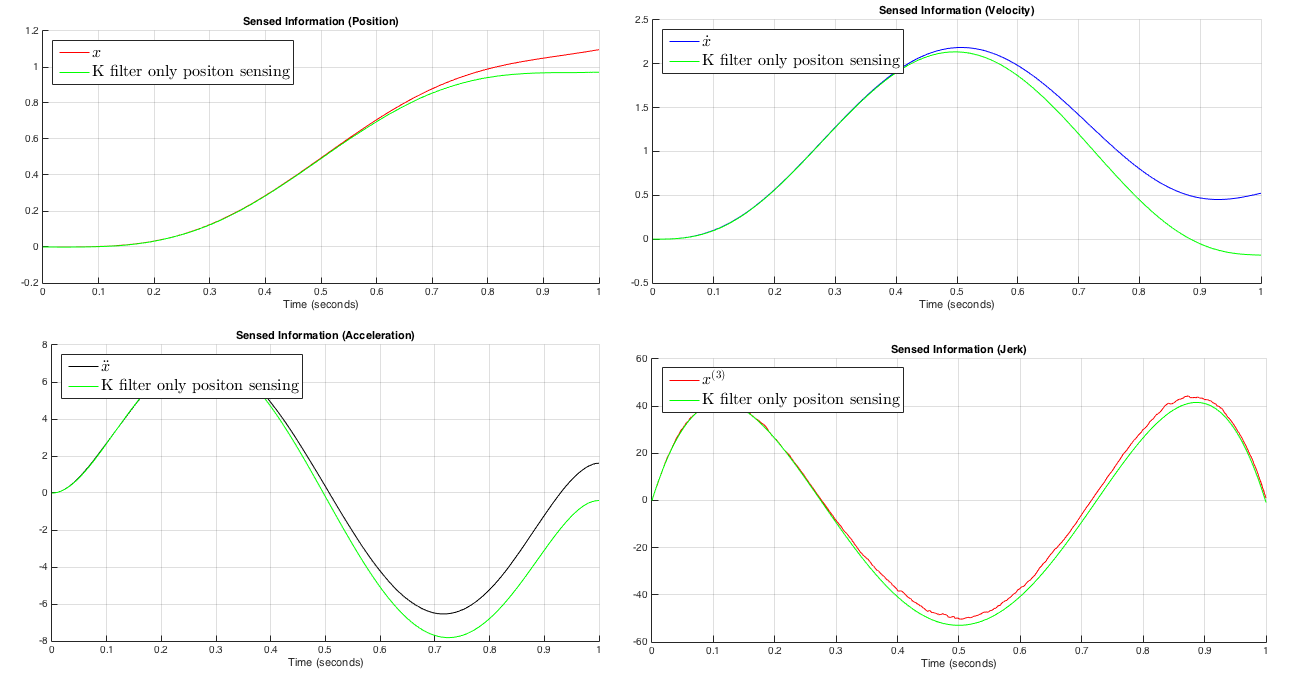
\includegraphics[width = \linewidth]{position_only}
\end{figure} 

\paragraph{Velocity, Acceleration, and Jerk}
	After running the Kalaman assignment multiple times I noticed there was no discernable difference between using only the velocity, acceleration, and jerk sensors and using all 4 sensors. However, I believe that if I continued plotting and measuring the error  using all 4 sensors would eventually out perform just using 3. Just using position was noticeably worse than the other two filters because filter can't compensate for error in the derivative terms. So ideally for a better Kalaman filter we would have as many sensors as possible, to get reliable sensor readings, and if we have to limit what kind of sensors, we would prefer sensors that can measure the derivative terms, rather than just position terms. 
\begin{figure}[!h]
\caption{Only using a Velocity , Acceleration, and Jerk Sensors}
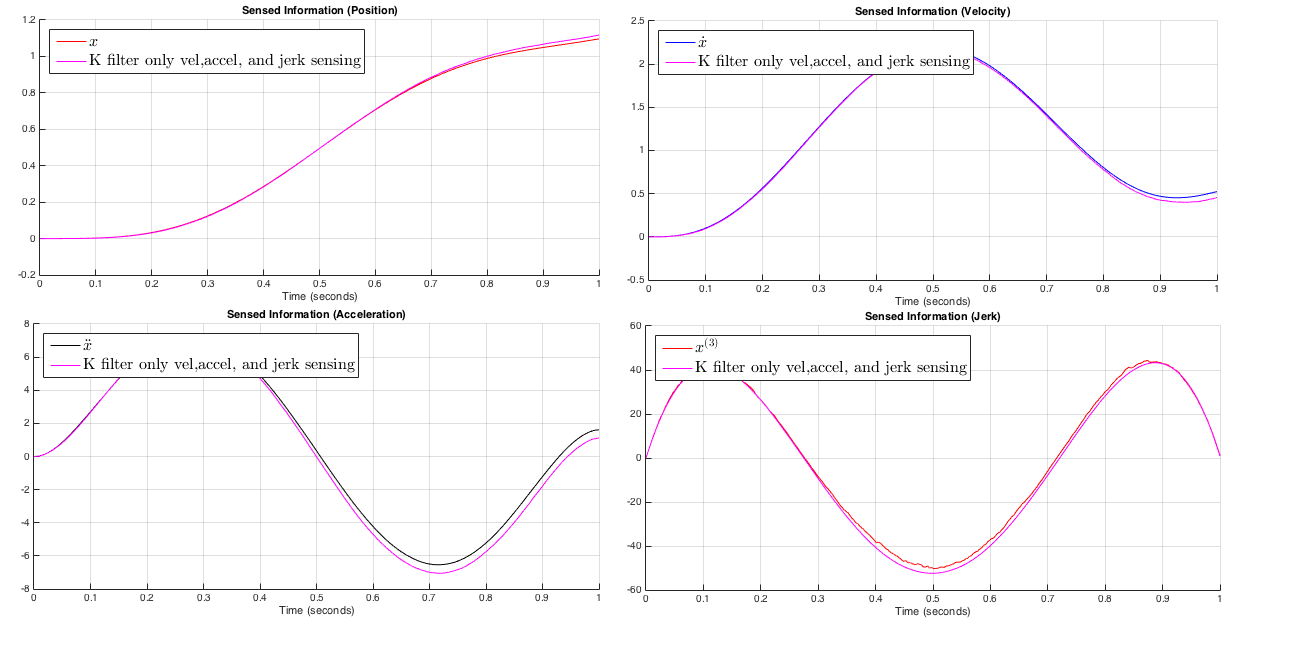
\includegraphics[width = \linewidth]{vaj}
\end{figure}  
 
 \begin{figure}[!h]
\caption{Using all 4 Sensors}
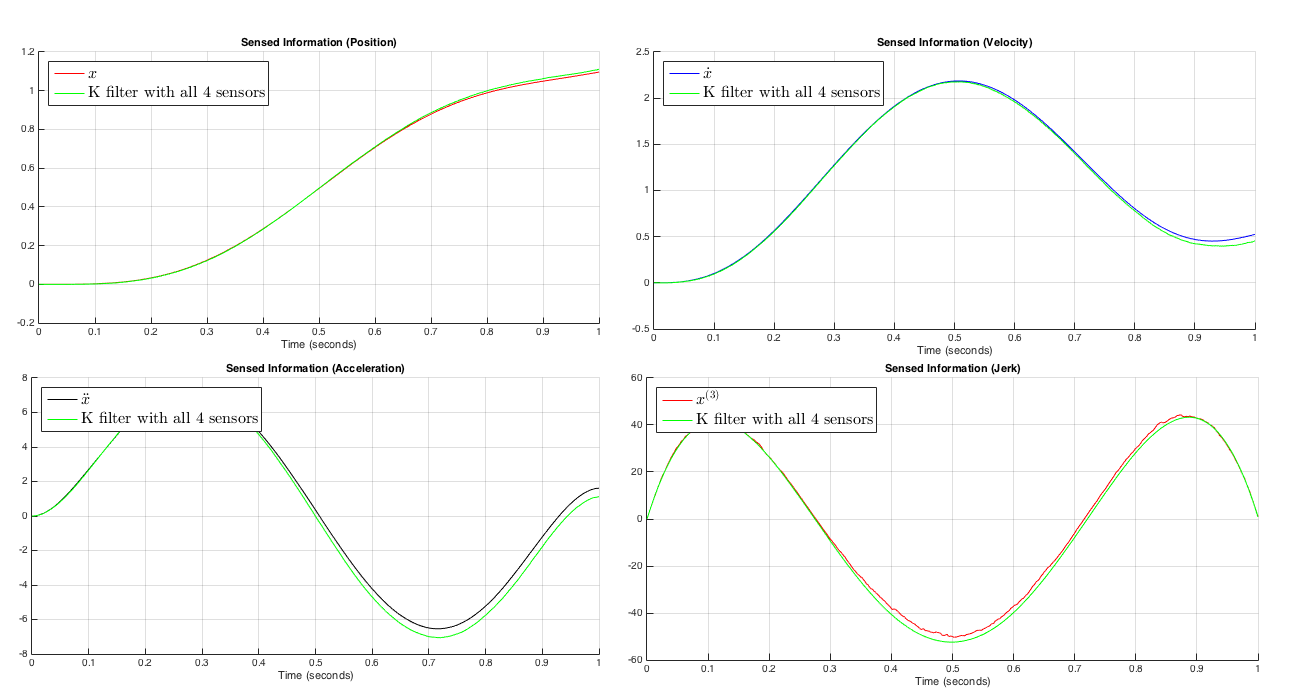
\includegraphics[width = \linewidth]{all4}
\end{figure}  
\end{document}
